\chapter{Introduction to Geometric Vectors}
\section{Definition and Operations of Geometric Vectors}

\subsection{Basic Structure of Vectors in the Real $n$-Space $\mathbb{R}^n$}
After three chapters of discussion about matrices, it is the time to talk about another concept that are pertinent to linear algebra, that are, vectors. A vector is a mathematical quantity represented by an ordered tuple of components (numbers), e.g. $(1, 8, 7, 4)$. It has a magnitude (length) and direction, resembling an arrow. Some real-life examples are: two-dimensional flow velocity $(u, v)$, relative position of an airplane to a ground radar $(x, y, z)$.\\
\\
A $m$-dimensional vector can be regarded as an $m \times 1$ (column vector) or $1 \times m$ matrix (row vector) and vice versa, depending on the situation. Usually the form of a column vector is more common than row vector.
\begin{defn}
A $m$-dimensional vector has $m$ ordered elements and are denoted by either an arrow or boldface, like $\vec{v}$ or $\textbf{v}$. It is defined as
\begin{align*}
\vec{v} &=
\begin{bmatrix}
v_1 \\
v_2 \\
v_3 \\
\cdots \\
v_m
\end{bmatrix}
=
(v_1, v_2, v_3, \cdots, v_m)^T
\end{align*}
\end{defn}
\begin{center}
\begin{tikzpicture}
\draw[->] (-2.5,0)--(2.5,0) node[right]{$x$};
\draw[->] (0,-2.5)--(0,2.5) node[above]{$y$};
\draw[blue,-stealth] (0,0)--(2,1) node[anchor=south west]{$\vec{v} = (2,1)^T$};
\draw[blue,dotted] (2,1)--(2,0) node[below]{$x = 2$};
\draw[blue,dotted] (2,1)--(0,1) node[left]{$y = 1$};
\node[below left]{$O$}; 
\end{tikzpicture}\\
A 2D vector in the x-y plane.
\end{center}
\begin{center}
\fbox{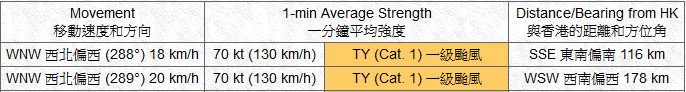
\includegraphics[scale = 0.5]{higos.jpg}}\\
Forecast for Typhoon Higos. (Taken from \href{http://www.hkww.org/weather/tcarchive.html}{here}) The movement is also a two-dimensional vectors, even though the speed and direction are given instead of the velocities in $x$ and $y$-direction.
\end{center}
Vectors can be written as the sum of unit vectors that have a length of $1$, denoted by $\hat{e}_p$, in the positive direction along the coordinates axes. They are referred to as the standard unit vectors, with $\hat{e}_1 = \hat{i} = (1,0,0)^T$, $\hat{e}_2 = \hat{j} = (0,1,0)^T$, $\hat{e}_3 = \hat{k} = (0,0,1)^T$ corresponding to $x$, $y$, $z$ axes respectively in three-dimensional settings.
\begin{defn}
The standard unit vector $\hat{e}_p$ consists of $1$ at the $p$-th entry and $0$ elsewhere.
\end{defn}
\begin{center}
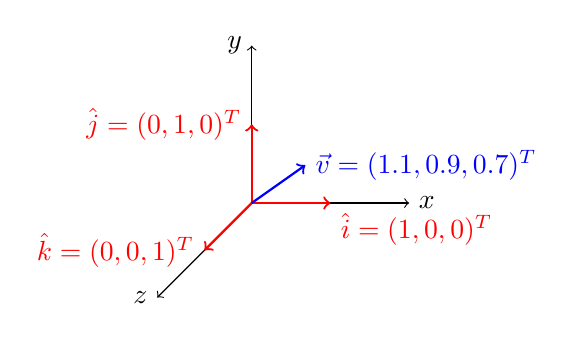
\begin{tikzpicture}[x=1cm, y=1cm, z=-0.6cm]
\draw [->] (0,0,0) -- (2,0,0) node [right] {$x$};
\draw [->] (0,0,0) -- (0,2,0) node [left] {$y$};
\draw [->] (0,0,0) -- (0,0,2) node [left] {$z$};
\draw [->, thick, red] (0,0,0) -- (1,0,0) node [below right] {$\hat{i} = (1,0,0)^T$};
\draw [->, thick, red] (0,0,0) -- (0,1,0) node [left] {$\hat{j} = (0,1,0)^T$} ; 
\draw [->, thick, red] (0,0,0) -- (0,0,1) node [left] {$\hat{k} = (0,0,1)^T$};
\draw [->, thick, blue] (0,0,0) -- (1.1,0.9,0.7) node [right] {$\vec{v} = (1.1,0.9,0.7)^T$};
\end{tikzpicture}
\begin{align*}
\vec{v} = 
\begin{bmatrix}
1.1 \\
0.9 \\
0.7
\end{bmatrix}
= 1.1
\begin{bmatrix}
1 \\
0 \\
0
\end{bmatrix}
+ 0.9
\begin{bmatrix}
0 \\
1 \\
0
\end{bmatrix}
+ 0.7
\begin{bmatrix}
0 \\
0 \\
1
\end{bmatrix}
&= 1.1\hat{i} + 0.9\hat{j} + 0.7\hat{k}\\
&= (1.1,0.9,0.7)^T
\end{align*}
\end{center}

\subsection{Vector Operations - Part I} 
\subsubsection{Addition and Subtraction}
Same as their matrix counterpart, Addition and subtraction between vectors is element-wise. Again, they are only valid for vectors of the same dimension. For $\vec{w} = \vec{u} \pm \vec{v}$, we have $w_i = u_i \pm v_i$. If
\begin{align*}
&\vec{u} =
\begin{bmatrix}
1 \\
2
\end{bmatrix}
&
\vec{v} =
\begin{bmatrix}
2 \\
-1
\end{bmatrix}
\end{align*}
then
\begin{align*}
\vec{u} + \vec{v} =
\begin{bmatrix}
\textcolor{red}{1} \\
\textcolor{red}{2}
\end{bmatrix}
+
\begin{bmatrix}
\textcolor{blue}{2} \\
\textcolor{blue}{-1}
\end{bmatrix}
&= 
\begin{bmatrix}
\textcolor{Green}{3} \\
\textcolor{Green}{1}
\end{bmatrix}
\\
\vec{u} - \vec{v} =
\begin{bmatrix}
\textcolor{red}{1} \\
\textcolor{red}{2}
\end{bmatrix}
-
\begin{bmatrix}
\textcolor{blue}{2} \\
\textcolor{blue}{-1}
\end{bmatrix}
&= 
\begin{bmatrix}
\textcolor{Green}{-1} \\
\textcolor{Green}{3}
\end{bmatrix}
\end{align*}
\begin{center}
\begin{tikzpicture}
\draw[->] (-3,0)--(3,0) node[right]{$x$};
\draw[->] (0,-3)--(0,3) node[above]{$y$};
\draw[red,-stealth] (0,0)--(1,2) node[anchor=south west]{$\vec{u} = (1,2)^T$};
\draw[blue,-stealth] (1,2)--(3,1) node[anchor=south west]{$\vec{v} = (2,-1)^T$};
\draw[Green,-stealth] (0,0)--(3,1) node[anchor=north west]{$\vec{u} + \vec{v} = (3,1)^T$};
\node[below left]{$O$}; 
\end{tikzpicture}\\
Addition: The tail of the blue vector is placed to the head of the red vector, and the resultant green vector is from the origin to the head of blue vector.
\begin{tikzpicture}
\draw[->] (-3,0)--(3,0) node[right]{$x$};
\draw[->] (0,-3)--(0,3) node[above]{$y$};
\draw[red,-stealth] (0,0)--(1,2) node[anchor=south west]{$\vec{u} = (1,2)^T$};
\draw[blue,-stealth] (1,2)--(-1,3) node[anchor=south east]{$-\vec{v} = (-2,1)^T$};
\draw[Green,-stealth] (0,0)--(-1,3) node[anchor=north east]{$\vec{u} - \vec{v} = (-1,3)^T$};
\node[below left]{$O$}; 
\end{tikzpicture}\\
Subtraction: Similar to addition but with the blue vector oriented in the opposite direction.
\end{center}

\subsubsection{Scalar Multiplication} 
Multiplying a scalar or number to a vector means that all components are multiplied by that scalar.
\begin{align*}
2
\begin{bmatrix}
2 \\
0 \\
1 \\
9
\end{bmatrix}
=
\begin{bmatrix}
4 \\
0 \\
2 \\
18
\end{bmatrix}
\end{align*}
From the previous discussion of vector subtraction, we know that subtraction can be viewed as addition with a $-1$ factor.
\begin{align*}
\begin{bmatrix}
7 \\
5 \\
9
\end{bmatrix}
-
\begin{bmatrix}
3 \\
6 \\
9
\end{bmatrix}
=
\begin{bmatrix}
7 \\
5 \\
9
\end{bmatrix}
+ (-1)
\begin{bmatrix}
3 \\
6 \\
9
\end{bmatrix}
=
\begin{bmatrix}
7 \\
5 \\
9
\end{bmatrix}
+
\begin{bmatrix}
-3 \\
-6 \\
-9
\end{bmatrix}
=
\begin{bmatrix}
4 \\
-1 \\
0
\end{bmatrix}
\end{align*}

\subsubsection{Length and Unit Vector} Length, or more formally Euclidean norm, of a vector $\vec{v}$ is based on a generalized version of Pythagoras’ Theorem, and is calculated as the square root of the sum of squares of components.
\begin{defn}
\label{vectorlength}
Length, or $2$-norm of a $m$-dimensional vector $\vec{v}$, denoted by $\norm{\vec{v}}$, is given by
\begin{align*}
\norm{\vec{v}} &= \sqrt{v_1^2 + v_2^2 + v_3^2 + \cdots + v_m^2} \\
&= \sqrt{\sum_{k=1}^{m} v_k^2}
\end{align*}
\end{defn}
Some illustrations are shown below.
\begin{center}
\begin{tikzpicture}
\draw[->] (-2.5,0)--(2.5,0) node[right]{$x$};
\draw[->] (0,-2.5)--(0,2.5) node[above]{$y$};
\draw[blue,-stealth] (0,0)--(2,1) node[anchor=south, shift={(12mm, 2.4mm)}]{$\norm{\vec{v}} = \sqrt{dx^2 + dy^2} = \sqrt{2^2+1^2} = \sqrt{5}$};
\draw[blue,dotted] (2,1)--(2,0) node[below]{$x = 2$};
\draw[blue,dotted] (2,1)--(0,1) node[left]{$y = 1$};
\node[below left]{$O$}; 
\end{tikzpicture}
\end{center}
\begin{align*}
&\vec{w} = 
\begin{bmatrix}
8 \\
-4 \\
1
\end{bmatrix}
& \norm{\vec{w}}=
\sqrt{8^2 + (-4)^2 + 1^2} = 9 
\end{align*}

The unit vector that has a length of $1$ and is in the same direction of some vector $\vec{v}$ is simply produced from dividing, or normalizing $\vec{v}$ by its distance $\norm{\vec{v}}$.
\begin{defn}
\label{unitvec}
The unit vector parallel to any non-zero vector $\vec{v}$ is denoted as $\hat{v}$ and is given by
\begin{align*}
\hat{v} &= \frac{1}{\norm{\vec{v}}}\vec{v}
\end{align*}
Unit vectors are all dimensionless when defined in this way.
\end{defn}
Short Exercise: Find a unit vector for $\vec{w}$ in the previous example, and verify that it has a length of $1$.

\subsection{Vector Operations - Part II}
\label{vectorops}
The next major vector operations we are going to introduce are two kinds of vector products, one is called the vector dot product, which is just a special case of the matrix dot product, another one is called the vector cross product. Some basic information about these two vector products are summarized below.
\begin{center}
\begin{tabular}{|p{30mm}|p{50mm}|p{15mm}|}
\hline
 & Input & Output \\
\hline
Dot Product, or Scalar Product ($\cdot$) & Two vectors, the order does not matter & A scalar\\
\hline
Cross Product, or Vector Product ($\times$) & Two three-dimensional vectors, the order is important & Another vector
\\
\hline
\end{tabular}
\end{center}

\subsubsection{Dot Product}
The dot product for any two vectors with the same dimension is the sum of products of paired components between the two vectors. In other words, it can be regarded as the matrix product between a row vector ($1 \times m$ matrix) and a column vector ($m \times 1$ matrix). Conversely, it can be said that entries of a matrix dot product are vector dot products between the corresponding row and column.
\begin{defn}
\label{dotreal}
Vector dot product between two $m$-dimensional vectors $\vec{u}$ and $\vec{v}$ are denoted as either $\vec{u} \cdot \vec{v}$, or by matrix notation $\textbf{u}^T\textbf{v}$. They are defined as
\begin{align*}
\vec{u} \cdot \vec{v} = \textbf{u}^T\textbf{v} &= u_1v_1 + u_2v_2 + u_3v_3 + \cdots + u_mv_m \\
&= \sum_{k=1}^{m} u_kv_k
\end{align*}
For Two matrices 
$A = [\vec{u}^{(1)}|\vec{u}^{(2)}|\cdots|\vec{u}^{(n)}]^T$,
$B = [\vec{v}^{(1)}|\vec{v}^{(2)}|\cdots|\vec{v}^{(n)}]$, their matrix product $AB$ can be written as
\begin{align*}
AB =
\begin{bmatrix}
\vec{u}^{(1)} \cdot \vec{v}^{(1)} & \vec{u}^{(1)} \cdot \vec{v}^{(2)} & \cdots & \vec{u}^{(1)} \cdot \vec{v}^{(n)} \\
\vec{u}^{(2)} \cdot \vec{v}^{(1)} & \vec{u}^{(2)} \cdot \vec{v}^{(2)} & \cdots & \vec{u}^{(2)} \cdot \vec{v}^{(n)} \\
\vdots & \vdots & & \vdots \\
\vec{u}^{(n)} \cdot \vec{v}^{(1)} & \vec{u}^{(n)} \cdot \vec{v}^{(2)} & \cdots & \vec{u}^{(n)} \cdot \vec{v}^{(n)} \\
\end{bmatrix}
\end{align*}
\end{defn}
As a consequence, length of a vector, as defined in Definition \ref{vectorlength}, can be written as the square root of dot product between the vector and itself.
\begin{proper}
\label{normpos}
The Euclidean norm of a vector can be written using its dot product as
\begin{align*}
\norm{\vec{v}} &= \sqrt{\vec{v} \cdot \vec{v}}\\
\norm{\vec{v}}^2 &= \vec{v} \cdot \vec{v}
\end{align*}
$\vec{v} \cdot \vec{v}$ is always greater than zero, unless when $\vec{v}$ is a zero vector, then $\vec{v} \cdot \vec{v} = 0$.
\end{proper}

\begin{exmp}
If $\vec{u} = (1, 2, 3, 4, 5)^T$ and $\vec{v} = (-1, 0, 1, 0, -1)^T$, find the dot product $\vec{u} \cdot \vec{v} = \textbf{u}^T\textbf{v}$.
\begin{align*}
\vec{u} \cdot \vec{v} &= (1)(-1) + (2)(0) + (3)(1) + (4)(0) + (5)(-1) = -3
\end{align*}
Alternatively,
\begin{align*}
\textbf{u}^T\textbf{v} &=
\begin{bmatrix}
1 & 2 & 3 & 4 & 5
\end{bmatrix}
\begin{bmatrix}
-1 \\
0 \\
1 \\
0 \\
-1
\end{bmatrix}
= -3
\end{align*}
\end{exmp}

Here are some properties of dot product.
\begin{proper}
\label{dotproper}
For three $m$-dimensional vectors $\vec{u}$, $\vec{v}$ and $\vec{w}$, the following establishes.
\begin{align*}
\vec{u} \cdot \vec{v} &= \vec{v} \cdot \vec{u} &\text{Commutative Property} \\
\vec{u} \cdot (\vec{v} \pm \vec{w}) &= \vec{u} \cdot \vec{v} \pm \vec{u} \cdot \vec{w} &\text{Distributive Property} \\
(\vec{u} \pm \vec{v}) \cdot \vec{w} &= \vec{u} \cdot \vec{w} \pm \vec{v} \cdot \vec{w} &\text{Distributive Property} \\
(a\vec{u}) \cdot (b\vec{v}) &= ab(\vec{u} \cdot \vec{v}) &\text{where $a$, $b$ are some constants}
\end{align*}
Additionally, if $A$ is an $n \times n$ square matrix, $n = m$, then
\begin{align*}
\vec{u} \cdot (A\vec{v}) &= \textbf{u}^T(A\textbf{v}) = (A^T\textbf{u})^T\textbf{v} = (A^T\vec{u}) \cdot \vec{v} \\
(A\vec{u}) \cdot \vec{v} &= (A\textbf{u})^T\textbf{v} = \textbf{u}^T(A^T\textbf{v}) = \vec{u} \cdot (A^T\vec{v})
\end{align*}
where we have used Properties \ref{transposeproper}.
\end{proper}
\begin{exmp}
For $\vec{u} = (1,3,1)^T$ and $\vec{v} = (2,-1,1)^T$, find $(\vec{u} + \vec{v}) \cdot (\vec{u} + \vec{v})$.
\\
By Properties \ref{dotproper}, we can rewrite the expression as
\begin{align*}
(\vec{u} + \vec{v}) \cdot (\vec{u} + \vec{v}) &= \vec{u} \cdot (\vec{u} + \vec{v}) + \vec{v} \cdot (\vec{u} + \vec{v}) \\
&= \vec{u} \cdot \vec{u} + \vec{u} \cdot \vec{v} + \vec{v} \cdot \vec{u} + \vec{v} \cdot \vec{v} \\
&= \vec{u} \cdot \vec{u} + 2 \vec{u} \cdot \vec{v} + \vec{v} \cdot \vec{v}
\end{align*}
Subsequently,
\begin{align*}
&\quad \vec{u} \cdot \vec{u} + 2 \vec{u} \cdot \vec{v} + \vec{v} \cdot \vec{v} \\
&= (1,3,1)^T \cdot (1,3,1)^T + 2((1,3,1)^T \cdot (2,-1,1)^T) + (2,-1,1)^T \cdot (2,-1,1)^T \\
&= (1^2 + 3^2 + 1^2) + 2((1)(2)+(3)(-1)+(1)(1)) + (2^2 + (-1)^2 + 1^2) \\
&= 11 + 2(0) + 6 \\
&= 17
\end{align*}
Alternatively, one can calculate $\vec{w} = \vec{u} + \vec{v} = (1,3,1)^T + (2,-1,1)^T = (3,2,2)^T$ and find $\vec{w} \cdot \vec{w} = \norm{\vec{w}}^2$ instead.
\end{exmp}
\begin{exmp}
Given $\vec{u}$ and $\vec{v}$ as defined in the example above, if
\begin{align*}
A =
\begin{bmatrix}
1 & 2 & 1 \\
2 & 0 & 3 \\
1 & 1 & -1
\end{bmatrix}
\end{align*}
verify that $\vec{u} \cdot (A\vec{v}) = (A^T\vec{u}) \cdot \vec{v}$.
\begin{align*}
A\vec{v} &= 
\begin{bmatrix}
1 & 2 & 1 \\
2 & 0 & 3 \\
1 & 1 & -1
\end{bmatrix}
\begin{bmatrix}
2 \\
-1 \\
1
\end{bmatrix} \\
&=
\begin{bmatrix}
(1)(2) + (2)(-1) + (1)(1) \\
(2)(2) + (0)(-1) + (3)(1) \\
(1)(2) + (1)(-1) + (-1)(1) 
\end{bmatrix} \\
&=
\begin{bmatrix}
1 \\
7 \\
0
\end{bmatrix} \\
\vec{u} \cdot (A\vec{v}) &= (1,3,1)^T \cdot (1,7,0)^T \\
&= (1)(1) + (3)(7) + (1)(0) \\
&= 22
\end{align*}
On the other hand,
\begin{align*}
A^T\vec{u} &= 
\begin{bmatrix}
1 & 2 & 1 \\
2 & 0 & 1 \\
1 & 3 & -1
\end{bmatrix}
\begin{bmatrix}
1 \\
3 \\
1
\end{bmatrix} \\
&=
\begin{bmatrix}
(1)(1) + (2)(3) + (1)(1) \\
(2)(1) + (0)(3) + (1)(1) \\
(1)(1) + (3)(3) + (-1)(1) 
\end{bmatrix} \\
&=
\begin{bmatrix}
8 \\
3 \\
9
\end{bmatrix} \\
(A^T\vec{u}) \cdot \vec{v} &= (8,3,9)^T \cdot (2,-1,1)^T \\
&= (8)(2) + (3)(-1) + (9)(1) \\
&= 22
\end{align*}
\end{exmp}

\subsubsection{Geometric Meaning of Dot Product}
The geometric meaning of vector dot product is embedded in the relation below.
\begin{proper}
\label{dotgeo}
For two vectors $\vec{u}$ and $\vec{v}$ which have the same dimension, we have
\begin{align*}
\vec{u} \cdot \vec{v} = \norm{\vec{u}}\norm{\vec{v}}\cos\theta
\end{align*}
where $\theta$ is the angle between $\vec{u}$ and $\vec{v}$.
\end{proper}
\begin{center}
\begin{tikzpicture}[scale=1.3]
\coordinate (0) at (0,0);
\draw[->](0)--(4,1) node[right](vecu){$\vec{u}$};
\draw[->](0)--(1,2) node[above](vecv){$\vec{v}$};
\draw[dotted] (1,2)--(24/17, 6/17);
\draw[red] (24/17+0.2, 6/17+0.05)--(24/17+0.15, 6/17+0.25)--(24/17-0.05, 6/17+0.2);
\pic[draw, ->, "$\theta$",angle eccentricity=1.5] {angle = vecu--0--vecv};
\draw[blue, very thick] (0,0)--(24/17, 6/17) node[below, shift={(0mm, -2mm)}]{$\norm{\vec{u}}\cos\theta$};
\end{tikzpicture}
\end{center}
If the absolute value of the dot product $|\vec{u} \cdot \vec{v}|$ is equal to $\norm{\vec{u}}\norm{\vec{v}}$, where $\vec{u}$ and $\vec{v}$ are non-zero vectors, then it implies that $\cos\theta = \pm 1$, $\theta$ is either $0$ or $\pi$, and hence the two vectors are parallel. In addition, we have the following observation.
\begin{proper}
\label{dotorth}
If the dot product between two vectors $\vec{u}$ and $\vec{v}$ is zero, so that $\vec{u} \cdot \vec{v} = \vec{v} \cdot \vec{u} = 0$, then by Properties \ref{dotgeo}, $\cos\theta = 0$ and $\theta$ between $\vec{u}$ and $\vec{v}$ is $\pi/2$, $\vec{u}$ and $\vec{v}$ are said to be perpendicular, or orthogonal. The converse is also true. Note that the zero vector is regarded to be orthogonal to any vector, so even if $\vec{u}$ or $\vec{v}$ is a zero vector, this properties still hold.
\end{proper}
Some may notice that as $-1 \leq \cos\theta \leq 1$, if $|\vec{u} \cdot \vec{v}| > \norm{\vec{u}}\norm{\vec{v}}$, then $\theta$ will be undefined. However, Cauchy–Schwarz Inequality ensures this will not happen.
\begin{thm}
\label{CauchySch}
Given two vectors $\vec{u}$ and $\vec{v}$ that are $m$-dimensional, Cauchy–Schwarz Inequality states that
\begin{align*}
|\vec{u} \cdot \vec{v}| &\leq \norm{\vec{u}}\norm{\vec{v}} \\
|u_1v_1+u_2v_2+\cdots+u_nv_n| &\leq \sqrt{u_1^2+u_2^2+\cdots+u_m^2}\sqrt{v_1^2+v_2^2+\cdots+v_m^2}
\end{align*}
\paragraph{Proof} Consider $\vec{w} = \vec{u} + t\vec{v}$, where $t$ is any number, then $\norm{\vec{w}}^2 = \vec{w}\cdot\vec{w}$ is a quadratic polynomial as
\begin{align*}
(\vec{u} + t\vec{v}) \cdot (\vec{u} + t\vec{v}) &= \norm{\vec{u}}^2 + 2t(\vec{u} \cdot \vec{v}) + t^2\norm{\vec{v}}^2
\end{align*}
by Properties \ref{dotproper}.
Now notice that with Properties \ref{normpos}
\begin{align*}
\norm{\vec{u}}^2 + 2t(\vec{u} \cdot \vec{v}) + t^2\norm{\vec{v}}^2 =(\vec{u} + t\vec{v}) \cdot (\vec{u} + t\vec{v}) = \norm{\vec{u} + t\vec{v}}^2 \geq 0    
\end{align*}
As it is a quadratic polynomial, if it is always greater than or equal to zero, i.e. has no root, it means that the determinant must be negative or zero. So,
\begin{align*}
\Delta &\leq 0 \\
(2(\vec{u} \cdot \vec{v}))^2 - 4\norm{\vec{u}}^2\norm{\vec{v}}^2 &\leq 0 \\
(\vec{u} \cdot \vec{v})^2 - \norm{\vec{u}}^2\norm{\vec{v}}^2 &\leq 0 \\
(\vec{u} \cdot \vec{v})^2 &\leq \norm{\vec{u}}^2\norm{\vec{v}}^2 \\
|\vec{u} \cdot \vec{v}| &\leq \norm{\vec{u}}\norm{\vec{v}}
\end{align*}
\end{thm}

\subsubsection{Cross Product}
Another crucial vector product is the cross product, which generates a new three-dimensional vector from two three-dimensional vectors as input. The new vector will be automatically orthogonal to the two input vectors, and the direction is determined by the right hand rule.
\begin{center}
\fbox{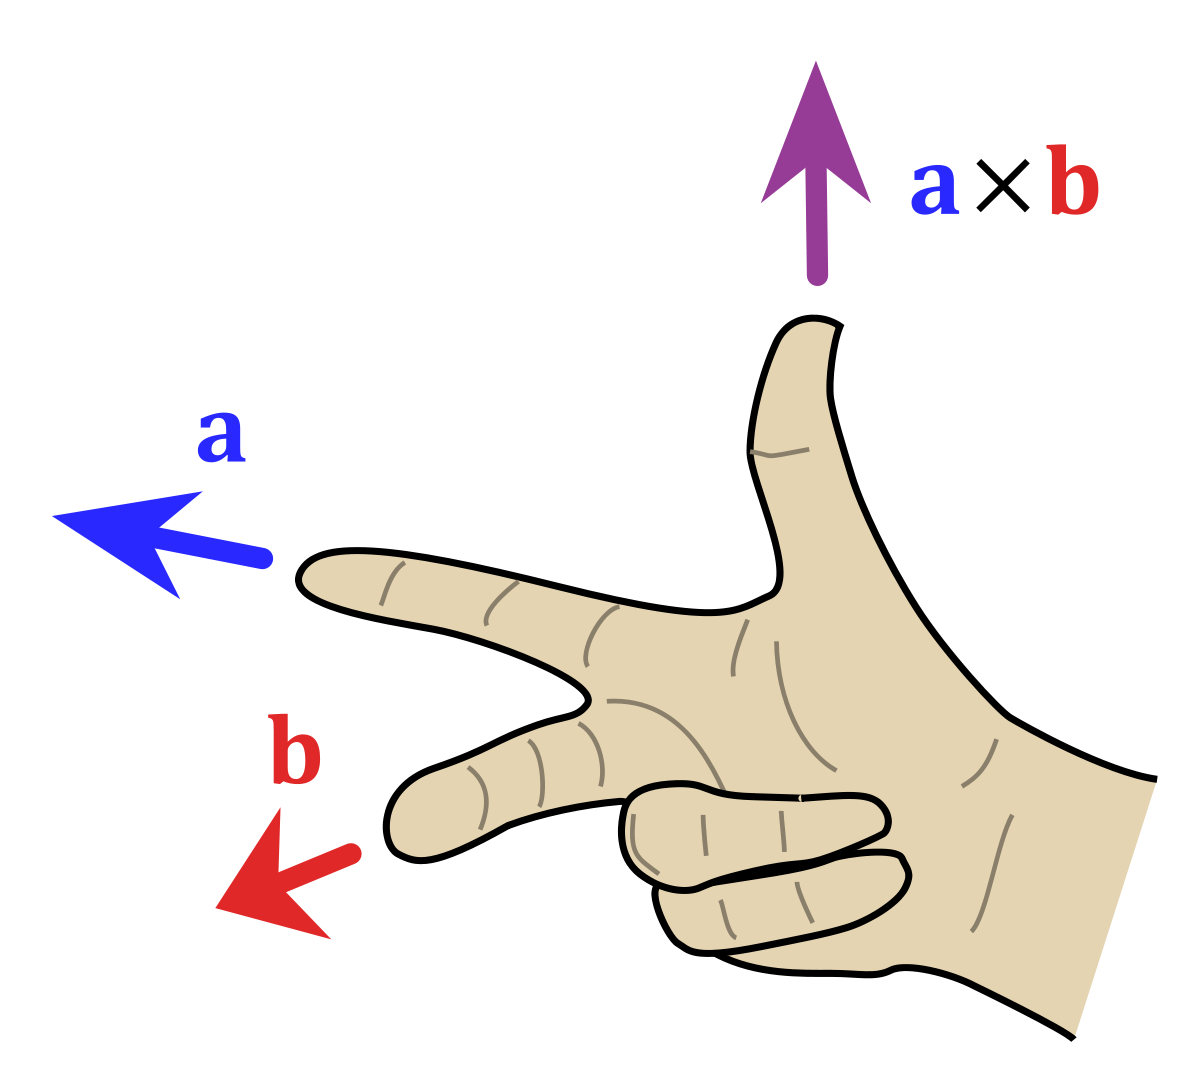
\includegraphics[scale = 0.1]{1200px-Right_hand_rule_cross_product.svg.png}}\\
Demonstration of the right hand rule. (Taken from Wikipedia)
\end{center}
The output of cross product is defined as
\begin{defn}
\label{crossdet}
For $\vec{u} = (u_1, u_2, u_3)^T$ and $\vec{v} = (v_1, v_2, v_3)^T$, the cross product $\vec{u} \times \vec{v}$ can be written in the form of a determinant as
\begin{align*}
\vec{u} \times \vec{v} =
\begin{vmatrix}
\hat{i} & \hat{j} & \hat{k} \\
u_1 & u_2 & u_3 \\
v_1 & v_2 & v_3
\end{vmatrix}
\end{align*}
\end{defn}

\begin{exmp}
Given two vectors
\begin{align*}
&\vec{u} =
\begin{bmatrix}
1 \\
0 \\
2
\end{bmatrix}
&\vec{v} =
\begin{bmatrix}
3 \\
-1 \\
1
\end{bmatrix}
\end{align*}
Find $\vec{u} \times \vec{v}$.
\begin{align*}
\vec{u} \times \vec{v} &=
\begin{vmatrix}
\hat{i} & \hat{j} & \hat{k} \\
1 & 0 & 2 \\
3 & -1 & 1
\end{vmatrix} \\
&= 
\hat{i}
\begin{vmatrix}
0 & 2 \\
-1 & 1 
\end{vmatrix}
- \hat{j}
\begin{vmatrix}
1 & 2 \\
3 & 1 
\end{vmatrix}
+ \hat{k}
\begin{vmatrix}
1 & 0 \\
3 & -1 
\end{vmatrix}
& \text{(Cofactor Expansion along the first row)} \\
&= 2\hat{i} + 5\hat{j} - \hat{k} = (2,5,-1)^T
\end{align*} 
Short Exercise: Check if $\vec{u} \times \vec{v}$ is orthogonal to $\vec{u}$ and $\vec{v}$ by finding the corresponding dot products.
\end{exmp}

Here are some useful observations about cross product.
\begin{defn}
\label{crosspr1}
Cross products involving the standard unit vectors $\hat{i}$, $\hat{j}$, $\hat{k}$ have the following rules.
\begin{enumerate}
\item $\hat{i} \times \hat{j} = \hat{k}$, $\hat{j} \times \hat{i} = -\hat{k}$,
\item $\hat{j} \times \hat{k} = \hat{i}$, $\hat{k} \times \hat{j} = -\hat{i}$,
\item $\hat{k} \times \hat{i} = \hat{j}$, $\hat{i} \times \hat{k} = -\hat{j}$.
\end{enumerate}
\end{defn}
\begin{center}
\fbox{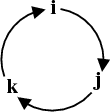
\includegraphics[scale = 0.5]{unit_vectors_cycle.png}}\\
A cyclic diagram for memorizing the above rules. Clockwise/anti-clockwise permutation results in positive/negative output. (Taken from \href{https://mathinsight.org/cross_product_formula}{here})
\end{center}
\begin{proper}
\label{crosspr2}
For two three-dimensional vectors $\vec{u}$ and $\vec{v}$, we have
\begin{align*}
\vec{u} \times \vec{v} &= -\vec{v} \times \vec{u} &\text{Anti-commutative Property} \\
\vec{u} \times (\vec{v} \pm \vec{w}) &= \vec{u} \times \vec{v} \pm \vec{u} \times \vec{w} &\text{Distributive Property} \\
(\vec{u} \pm \vec{v}) \times \vec{w} &= \vec{u} \times \vec{w} \pm \vec{v} \times \vec{w} &\text{Distributive Property} \\
(a\vec{u}) \times (b\vec{v}) &= ab(\vec{u} \times \vec{v}) &\text{where $a$, $b$ are some constants}
\end{align*}
\end{proper}
Actually, Definition \ref{crosspr1} and Properties \ref{crosspr2} together give rise to the determinant formula in Definition \ref{crossdet}. 

\subsubsection{Geometric Meaning of Cross Product} Similar to vector dot product, vector cross product has a geometric interpretation.
\begin{proper}
\label{crossgeo}
Given two vectors $\vec{u}$ and $\vec{v}$ which are both three-dimensional, the magnitude of $\vec{u} \times \vec{v}$ is related to the angle between $\vec{u}$ and $\vec{v}$ as
\begin{align*}
\norm{\vec{u} \times \vec{v}} = \norm{\vec{u}}\norm{\vec{v}}\sin\theta
\end{align*}
\end{proper}
Immediately, we know that if $\vec{u}$ and $\vec{v} = k\vec{u}$, where $k$ is some constant, are parellel, their cross product will be a zero vector, or equivalently $\vec{u} \times \vec{u} = \textbf{0}$. This can be proved via writing out the determinant form as well.

\begin{exmp}
If $\vec{u} = (1,2,3)^T$, and $\vec{v} = (-1,1,0)^T$, find $(\vec{u} + 2\vec{v}) \times (\vec{u} - \vec{v}) $.\\
\\
Observe that
\begin{align*}
(\vec{u} + 2\vec{v}) \times (\vec{u} - \vec{v}) &= \vec{u} \times (\vec{u} - \vec{v}) + 2\vec{v} \times (\vec{u} - \vec{v}) \\
&= \vec{u} \times \vec{u} - \vec{u} \times \vec{v} + 2\vec{v} \times \vec{u} - 2\vec{v} \times \vec{v} \\
&= -3\vec{u} \times \vec{v}
\end{align*}
where the fact that $\vec{u} \times \vec{u} = 0$, $\vec{v} \times \vec{v} = 0$ and Properties \ref{crosspr2} are used. Now,
\begin{align*}
-3\vec{u} \times \vec{v} &=  
-3
\begin{vmatrix}
\hat{i} & \hat{j} & \hat{k} \\
1 & 2 & 3 \\
-1 & 1 & 0
\end{vmatrix} \\
&= -3\left(\hat{i}
\begin{vmatrix}
2 & 3 \\
1 & 0 
\end{vmatrix}
- \hat{j}
\begin{vmatrix}
1 & 3 \\
-1 & 0 
\end{vmatrix}
+ \hat{k}
\begin{vmatrix}
1 & 2 \\
-1 & 1 
\end{vmatrix}\right) \\
&= -3(-3\hat{i}-3\hat{j}+3\hat{k}) \\
&= 9\hat{i}+9\hat{j}-9\hat{k} = (9,9,-9)^T
\end{align*}
\end{exmp}

Finally, cancellation of dot product or cross product at both sides of an equation is generally not correct.

\section{Exercises}

\begin{Exercise}
For $\vec{u} = (1, 3, 3, 7)^T$ and $\vec{v} = (1, 2, 2, 5)^T$, find
\begin{enumerate}[label=(\alph*)]
\item $\vec{u} + \vec{v}$,
\item $\frac{3}{2}\vec{u} - \frac{1}{2}\vec{v}$,
\item $\vec{u} \cdot \vec{v}$,
\item $\vec{v} \cdot \vec{u}$,
\item $(\vec{u} - 2\vec{v}) \cdot (2\vec{u} + \vec{v})$.
\end{enumerate}
\end{Exercise}

\begin{Exercise}
For $\vec{u} = (7, 4, 1)^T$, $\vec{v} = (8, 1, 1)^T$, and
\begin{align*}
A = 
\begin{bmatrix}
1 & 1 & 1\\
0 & 1 & 1\\
0 & 0 & 1
\end{bmatrix}
\end{align*}
Verify that
\begin{enumerate}[label=(\alph*)]
\item $(\vec{u} + \vec{v}) \cdot (\vec{u} - \vec{v}) = \vec{u} \cdot \vec{u} - \vec{v} \cdot \vec{v}$,
\item $\vec{u} \times \vec{v} = -\vec{v} \times \vec{u}$, 
\item $\vec{u} \cdot (\vec{Av}) = (A^T\vec{u}) \cdot \vec{v}$, and
\item Compute $(3\vec{u} - 4\vec{v}) \cdot (\vec{u} \times \vec{v})$, is the answer what you expect?
\end{enumerate}
\end{Exercise}

\begin{Exercise}
For $\vec{u} = (1, -3, 9)^T$ and $\vec{v} = (1, -2, 4)^T$, find
\begin{enumerate}[label=(\alph*)]
\item Their unit vectors $\hat{u}$ and $\hat{v}$,
\item The angle between them, by calculating their dot product,
\item The cross product $\vec{u} \times \vec{v}$, and 
\item Prove that the vector obtained from the cross product above is orthogonal (perpendicular) to $\vec{u}$ and $\vec{v}$, by calculating the corresponding dot products.
\end{enumerate}
\end{Exercise}

\begin{Exercise}
The following table contains incomplete data about the movement of several typhoons at some moments. Complete the table by filling in the blanks. The first one has been done as an example.
\begin{center}
\begin{tabular}{|c|c|c|c|c|}
\hline
Typhoon Name & Time & Speed & Direction & Vector Form\\
\hline
Nuri & 2008/08/22, 08:00 & \SI{13}{\km \per \hour} & NW ($\sim \SI{315}{\degree}$) & $(-9.192, 9.192)$\\
\hline
Vicente & 2012/07/24, 02:00 & \SI{18}{\km \per \hour} & \SI{299}{\degree} & \\
\hline
Linfa & 2015/07/09, 23:00 & & & $(-13.595, -6.339)$\\
\hline
Mangkhut & 2018/09/16, 22:00 & & \SI{288}{\degree} & $(\quad, 7.725)$\\
\hline
\end{tabular}
\end{center}
\end{Exercise}

\begin{Exercise}
Prove Cosine Law with vector notation by considering the triangle below
\begin{center}
\begin{tikzpicture}
\coordinate (0) at (0,0);
\draw[red,-{Latex[length=5mm, width=2mm]}] (0)--(5,1) node[right]{$\vec{u}$};
\draw[blue,-{Latex[length=5mm, width=2mm]}] (0)--(1,3) node[above]{$\vec{v}$};
\draw[Green,-{Latex[length=5mm, width=2mm]}] (1,3)--(5,1) node[midway, above, shift={(0mm, 3mm)}]{$\vec{u} - \vec{v}$};
\end{tikzpicture}
\end{center}
and expanding the quantity $\norm{(\vec{u}-\vec{v})}^2 = (\vec{u}-\vec{v}) \cdot (\vec{u}-\vec{v})$.
\end{Exercise}

\begin{Exercise}
The Coriolis effect is a phenomenon describing the deflection of motion due to the rotation of the Earth. Define the rotating frame of reference with the $x$-direction being the zonal direction, $y$-direction being the meridional direction, and $z$-direction being the zenith direction (normal to the Earth's surface), then the acceleration is given by $\vec{a} = -f (\hat{k} \times \vec{v})$, where $f = 2\Omega\sin{\varphi}$, $\Omega = \SI{7.292e-5}{\radian \per \s}$ is the angular speed of Earth's rotation, $\varphi$ is the latitude, and $\vec{v}$ is the velocity vector projected onto the horizontal $(v_x, v_y, 0)$ (or $(u, v, 0)$). Find the Coriolis acceleration in vector form for the following cases:
\begin{enumerate}[label=(\alph*)]
\item $\varphi = \SI{15}{\degree}$, $v_x = \SI{4}{\m \per \s}$s, $v_y = \SI{3}{\m \per \s}$,
\item $\varphi = -\SI{30}{\degree}$, $v_x = \SI{5}{\m \per \s}$, $v_y = -\SI{12}{\m \per \s}$, and
\item $\varphi = \SI{45}{\degree}$, $v_x = (2\sin{t})\si{\m \per \s}$, $v_y = (1 + \cos{t}) \si{\m \per \s}$, for $0 \leq t \leq 2\pi$, also (Calculus required) express the magnitude (length) of the acceleration vector in terms of $\cos t$, and find its maximum.
\end{enumerate}
\begin{center}
\fbox{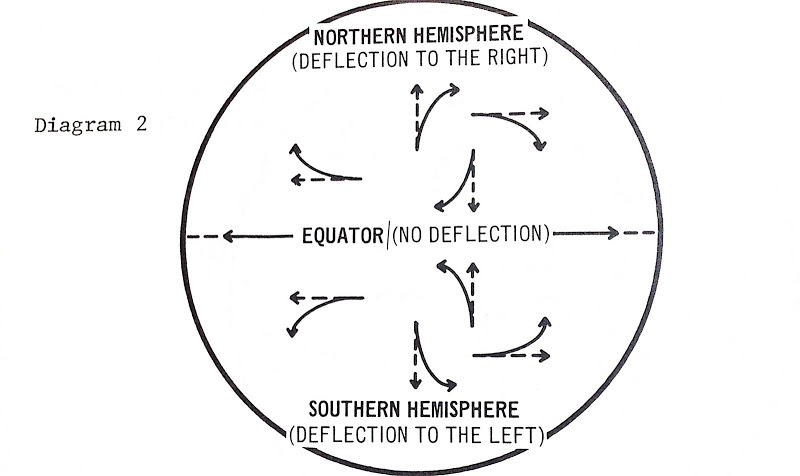
\includegraphics[scale = 0.4]{Coriolis.jpg}} \\
(Unknown Origin)
\end{center}
\end{Exercise}